%
%   Talk to be presented at the MPI developers conference in 
%  June 1995 at Notra Dame.
%
\def\stripe{\ifvmode\else\par\vskip-\baselineskip\vskip12pt\fi
\hbox to \hsize{\leaders\hrule height 4.5pt\hfil}\vskip-\baselineskip
            \vskip 3.5pt 
            \hbox to \hsize{\leaders\hrule height 1.5pt\hfil}
            \vskip -10pt}
\def\vt{\protect\begin{slide}}
\def\ve{\vfil\protect\end{slide}}
\def\vtt#1{\begin{slide}{}{\bf #1}\stripe\vfil\parskip8pt}
\def\vttstar#1{\begin{slide*}{}{\bf #1}\stripe\vfil\parskip8pt}
\def\vestar{\vfil\protect\end{slide*}}

\documentstyle[psfig]{seminar}
\landscapeonly

\begin{document}

\vt

\vspace{.6in}

\begin{center}
{\Large PETSc 2.0} \\
{\Large MPI Based Numerical Libraries}\\
\end{center}

\begin{center}
William Gropp\\
Lois Curfman McInnes \\
Barry Smith\\
http://www.mcs.anl.gov/petsc/petsc.html\\
\end{center}
\vspace{0cm}
\centerline{\hspace{.75in} 
\psfig{file=../argonne.ps,height=1.7in,width=1.7in}}
\ve

\vt
\vspace{.2in}
\centerline{\hspace{3.6in} \psfig{file=../petsc_pt.eps,height=5.1in,width=7.9in}}
\ve



\vtt{General Contents: PETSc Objects}
\begin{itemize}
\item vectors
\item matrices (sparse and dense)
\item Krylov subspace solvers
\item classical preconditioners
\item Newton based nonlinear solvers
\item distributed Arrays
\item distributed grids
\item simple graphics
\end{itemize}
\ve

\vtt{History of PETSc}

\vspace{1in}

September 1991, PETSc begun including Chameleon light-weight
 message-passing system.

September 1994, PETSc 2.0 begun.

June 1995, first general beta release of PETSc 2.0 for MPI.
\ve


\vtt{Design Features}
ANSI C (Could have used C++)

Data encapsulation (Data hiding)

Polymorphism (e.g., one uses {\tt MatMult()} regardless of the matrix 
              data structure)

Dynamic (run-time) binding of functions

Context variables

Very limited inheritance, from base PETSc object
\ve

%
% verbatim don't work with seminar.sty ^&%^&%^&
%
\vtt{Design Features: A Peek Inside a Vector}
{\tiny 
\begin{tabbing} 
struct \= \_PetscHeader \{ \\
\>  MPI\_Comm \=   comm;  \kill
\>  int  \>       cookie; \\                     
\>  int  \>       (*destroy)(PetscObject);\\     
\>  ....\\
\>  MPI\_Comm  \>  comm;  \\                      
\};\\
struct \_VeOps \{\\
\>  int \> (*duplicate)(Vec,Vec*),           /*  Get single vector */\\
\> \>       (*dot)(Vec,Vec,Scalar*),          /*  z = x\^H * y */\\
\> \>       (*mdot)(int,Vec,Vec*,Scalar*),    /*  z[j] = x dot y[j] */\\
\>       ...\\
\};\\
struct \_Vec \{\\
\> struct \> \_PetscHeader \= header;\\
\>  struct \> \_VeOps      \> *ops;\\
\>  void \>              \>  *data;\\
\};\\
typedef struct \{ int n; Scalar *array; \} Vec\_Seq;\\
typedef struct \_Vec* Vec;
\end{tabbing}}
\ve


\vtt{Why C? (C++ could also be a reasonable approach)}
Because we could.

Users have full access to PETSc objects from Fortran, C, and C++.

Portability. 

A standard, reliable language.

Would have to work on the boundaries of C++, which is 
a rapidly developing language, when we need a strong, 
static, reliable platform.
\ve

\vtt{Parallelism in PETSc}
Message-passing, but often the use of PETSc objects 
leads to SIMD type application code.

Much of message passing is hidden from users.

Will discuss several PETSc objects.
\ve


\vtt{Vectors}
PETSc provides all expected operations:

\[
x = a*x + y \hspace{.8in} y = a*x + y \hspace{.8in} w = a*x + y
\]

\[
d = x \cdot y \hspace{.8in} \hbox{VecDuplicate()} \hspace{.8in} 
   \hbox{VecDestroy()}
\]

{\bf Easy} parallel vector assembly.

{\bf Easy} parallel vector scatters.

\ve

\vtt{Matrices}
PETSc provides many of the expected operations:

\[
y = A *x \hspace{.8in} y = A^{T} x
\]

{\bf Easy} parallel matrix assembly. 

Support for several simple preconditioners.

Several different possible sparse representations.
\ve


\vtt{Overlapping Communication and Computation}
Must be {\bf easy} and natural in application level code.

BeginPetscOperation(...)

/* other work */

EndPetscOperation(...)

\ve

\vtt{Case Study: Vector Assembly}
...

/* each processors generates whichever values it pleases */

VecSetValues(Vec vec,int n,int *indices,Scalar *values);

...

VecAssemblyBegin(Vec);

/* do other useful work */

VecAssemblyEnd(Vec);
\ve

\vtt{Case Study: Vector Assembly (continued)}
{\small 
\begin{tabbing}
double \= x0, y0, x1, y1, x2, y2, f[3];\\
int \>  i, n[3];\\
         /* loop over local elements */\\
          for \=( i=0; i$<$Nt; i++ ) \{\\
    \>         n[0] = tri[3*i];  n[1] = tri[3*i+1];  n[2] = tri[3*i+1];\\
    \>         x0 = XY[6*i];     y0 = XY[6*i+1]; \\
    \>         x1 = XY[6*i+2];   y1 = XY[6*i+3]; \\
    \>         x2 = XY[6*i+4];   y2 = XY[6*i+5]; \\
   \>          CalculateElementIntegral(n,x0,x1,x2,y0,y1,y2,f);\\
   \>          VecSetValues(F,3,n,f,ADDVALUES);\\
          \}\\
           VecAssemblyBegin(F);\\
          VecAssemblyEnd(F);\\
          return 0;\\
\end{tabbing}}
\ve

\vtt{Phases in Vector Assembly}
Each processor
\begin{itemize}
\item Determines maximum size delivery to expect,
      as well as  number of deliveries, using
      calls to {\tt MPI\_Allreduce()}. 
\item Allocates buffers for all the stashed values
      to arrive in and posts corresponding nonblocking receives.
\item Posts nonblocking sends of all the elements to 
      be distributed.
\stripe
\item Waits for its receives and inserts the received 
      values into the correct locations as indicated by the received
      indices.
\item Finally, all processors wait on their nonblocking sends.
\end{itemize}

\ve

\vtt{Case Study: Vector Scatter (add)}
\begin{tabbing}
        VecScatterCtx \= ctx; \\
        IS       \>     isfrom, isto;\\
        ISCreateStride(MPI\_Comm comm,n/2,0,1,\&isto);\\
        ISCreateStride(MPI\_Comm comm,n/2,0,2,\&isfrom);\\
        VecScatterCtxCreate(xfrom,isfrom,xto,isto,\&ctx);\\
        ISDestroy(isto); ISDestroy(isfrom);\\
        VecScatterBegin(xfrom,xto,INSERT,SCATTER,ctx);\\
        /* do other useful work */\\
        VecScatterEnd(xfrom,xto,INSERT,SCATTER,ctx);\\
\end{tabbing}

It would be nice if MPI had receive-add (or a more general 
receive-operation). 
\ve

\vtt{Phases in {\tt VecScatterCreate}}
Each processor
\begin{itemize}
\item Determine maximum size delivery to expect
      as well as  number of deliveries, using
      calls to {\tt MPI\_Allreduce()}. 
\item Allocates index buffers for requested indices
      to arrive in and posts corresponding nonblocking receives.
\item Posts nonblocking sends of all the required indices.
\stripe
\item Waits for its receives and inserts the received 
      indices into {\tt VecScatterCtx} buffers.
\item Finally, all processors wait on their nonblocking sends.
\end{itemize}

\ve

\vtt{Case Study: Matrix-vector multiply}
\begin{tabbing}
For a row storage based sparse matrix.\\
       int \= MatMult\_MPIAIJ(Mat A,Vec x,Vec y)\\
        \{\\
    \>      Mat\_MPIAIJ *aij = (Mat\_MPIAIJ *) A-$>$data;\\
    \>      VecScatterBegin(x,aij-$>$lvec,INSERT,SCATTER,aij-$>$Mvctx);\\
    \>      MatMult(aij-$>$A,x,y);\\
    \>      VecScatterEnd(x,aij-$>$lvec,INSERT,SCATTER,aij-$>$Mvctx);\\
    \>      MatMultAdd(aij-$>$B,aij-$>$lvec,y,y);\\
    \>      return 0;\\
        \}
\end{tabbing}
\ve

\vtt{Case Study: Matrix-vector multiply (continued)}
\begin{tabbing}
int \= MatMultTrans\_MPIAIJ(Mat aijin,Vec xx,Vec yy)\\
\{\\
 \>  Mat\_MPIAIJ *aij = (Mat\_MPIAIJ *) aijin-$>$data;\\
 \> MatMultTrans(aij-$>$B,xx,aij-$>$lvec);\\
 \> /* send it on its way */ \\
 \> VecScatterBegin(aij-$>$lvec,yy,ADDVALUES,RSCATTER,aij-$>$Mvctx);\\
 \> /* do local part */\\
 \> MatMultTrans(aij-$>$A,xx,yy);\\
 \> /* receive remote parts:  */ \\
 \> VecScatterEnd(aij-$>$lvec,yy,ADDVALUES,RSCATTER,aij-$>$Mvctx);\\
\>  return 0;\\
\}
\end{tabbing}
\ve

\vtt{Simple Distributed Arrays}

\vspace{1cm} 

\centerline{\hspace{3.6in} 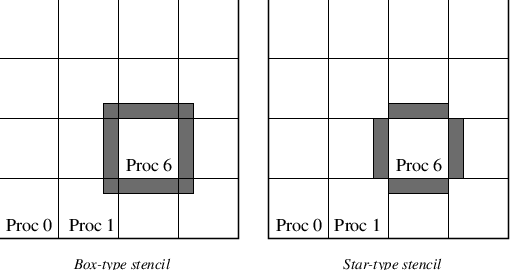
\psfig{file=../papers/ghost.eps,height=3in,width=7in,angle=0}}


\vspace{-1.7in}

{\small
\begin{tabbing}
DACreate2d(MPI\_Comm,\=DA\_STENCIL\_BOX,int M, int N, int m, int n, \\
                    \> int w, int s, DA *da);\\
DACreate2d(MPI\_Comm,DA\_STENCIL\_STAR,int M, int N, int m, int n, \\
                    \> int w, int s, DA *da);
\end{tabbing}}
\ve

\vtt{Simple Distributed Arrays: Usage}
{\small
\begin{tabbing}
          /* Transfer local portion of vector into a local work \\
             array, including ghost points */\\
          DAGlobalToLocalBegin(user-$>$da,X,INSERTVALUES,localX);\\
          /* do other useful work */\\
          DAGlobalToLocalEnd(user-$>$da,X,INSERTVALUES,localX);\\
          VecGetArray(localX,\&x); VecGetArray(localF,\&f);\\
          DAGetCorners(user-$>$da,\&xs,\&ys,0,\&xm,\&ym,0);\\
          DAGetGhostCorners(user-$>$da,\&Xs,\&Ys,0,\&Xm,\&Ym,0);\\
          for \= (j=ys; j$<$ys+ym; j++) \{\\
    \>        for \= (i=xs; i$<$xs+xm; i++) \{\\
    \> \>           /* operate on local values */\\
    \>        \}\\
          \}\\
          /* stick values into global vector */\\
          DALocalToGlobal(user-$>$da,localF,INSERTVALUES,F);
\end{tabbing}}
\ve



\vtt{Conclusion: Go with MPI!}
{\bf Don't} just add MPI to your list of supported 
message-passing systems.

{\bf Jettison} all support for other message-passing systems.\\
1) You save all the work of maintaining your own portability system.\\
2) You can take advantage of all of the unique and special 
   capabilities of MPI. 

PETSc previously included the Chameleon message-passing system. That is
now completely removed from PETSc 2.0. PETSc 2.0, as a result, is 
much smaller and easier to maintain and understand.
 
{\bf Do it today! There is no reason not to!}
\ve

\end{document}
